\RequirePackage[l2tabu, orthodox]{nag}
%\documentclass[12pt]{article}
\documentclass[preprint,12pt,times]{elsarticle}

% \usepackage{url}

% \usepackage[linesnumbered,lined,commentsnumbered,ruled]{algorithm2e}
%\usepackage{amssymb}
\usepackage{amsmath}
%\usepackage{amsfonts}
\usepackage{bm}
%\usepackage{bbm}
%\usepackage{caption}
\usepackage{xcolor}
%\usepackage{geometry}
%\usepackage{graphicx}
%\usepackage[colorlinks,linkcolor=blue,citecolor=blue,urlcolor=blue]{hyperref}
\usepackage{listings}
\lstset{ %
   backgroundcolor=\color{white},   % choose the background color; you must add \usepackage{color} or \usepackage{xcolor}
   basicstyle=\small,        % the size of the fonts that are used for the code
   breakatwhitespace=false,         % sets if automatic breaks should only happen at whitespace
   breaklines=false,                 % sets automatic line breaking
   captionpos=b,                    % sets the caption-position to bottom
   %commentstyle=\color{mygreen},    % comment style
   deletekeywords={...},            % if you want to delete keywords from the given language
   escapeinside={\%*}{*)},          % if you want to add LaTeX within your code
   extendedchars=false,              % lets you use non-ASCII characters; for 8-bits encodings only, does not work with UTF-8
   frame=single,	                   % adds a frame around the code
   keepspaces=true,                 % keeps spaces in text, useful for keeping indentation of code (possibly needs columns=flexible)
   keywordstyle=\color{blue},       % keyword style
   language=C++,                 % the language of the code
   otherkeywords={*,...},           % if you want to add more keywords to the set
   numbers=left,                    % where to put the line-numbers; possible values are (none, left, right)
   numbersep=5pt,                   % how far the line-numbers are from the code
   numberstyle=\tiny\color{gray}, % the style that is used for the line-numbers
   rulecolor=\color{black},         % if not set, the frame-color may be changed on line-breaks within not-black text (e.g. comments (green here))
   showspaces=false,                % show spaces everywhere adding particular underscores; it overrides 'showstringspaces'
   showstringspaces=false,          % underline spaces within strings only
   showtabs=false,                  % show tabs within strings adding particular underscores
   stepnumber=2,                    % the step between two line-numbers. If it's 1, each line will be numbered
%   stringstyle=\color{mymauve},     % string literal style
   tabsize=2,	                   % sets default tabsize to 2 spaces
   title=\lstname                   % show the filename of files included with \lstinputlisting; also try caption instead of title
}
%\usepackage{layouts}
%\usepackage{mathrsfs}
%\usepackage{pgfkeys,pgfmath,pgfcore}
%\usepackage{srcltx}
%\usepackage[labelformat=simple]{subcaption}
%\usepackage{xspace}
\usepackage[linesnumbered,lined,commentsnumbered,ruled]{algorithm2e}

\usepackage[format=plain,indention=.5cm]{caption}
\usepackage[labelformat=simple]{subcaption}
\renewcommand\thesubfigure{(\alph{subfigure})}

%\renewcommand{\thetable}{\arabic{table}}
%\captionsetup[table]{labelformat=simple, labelsep=colon}

%\pgfkeys{/pgf/number format/.cd,1000 sep={}}

%% see http://tex.stackexchange.com/questions/2441/how-to-add-a-forced-line-break-inside-a-table-cell
%\newcommand{\specialcell}[2][c]{%
%  \begin{tabular}[#1]{@{}c@{}}#2\end{tabular}}

% put your own definitions here:
% \renewcommand\thesubfigure{(\alph{subfigure})}
\def\gz  #1{           \mbox{$\boldsymbol{#1}$}}
% \DeclareMathAlphabet{\bsf}{OT1}{cmss}{bx}{n}
% \def\msf  #1{           \mbox{\!\!      $\sf #1$}}
% \def\Grad #1 {{\rm Grad} #1}
% \def\grad #1 {{\rm grad} #1}
\def\Div {\mbox{Div\,}}
\def\div {\mbox{div\,}}
\def\d {\,\mbox{d}}
\def\D {\,\mbox{D}}
% \newcommand{\norm}[1]{\left\lvert #1 \right\rvert}
%\newcommand\normDouble[1]{\left\lVert#1\right\rVert}
%\newcommand{\normXY}[1]{\lvert #1 \rvert_{2d}}
%\newcommand{\dbracket}[1]{\left[\!\!\left[ #1 \right]\!\!\right]}

\def\mcl  #1{               {\cal #1}}
%\def\bcl  #1{\mbox{\boldmath$\cal #1$}}

%\DeclareMathOperator{\det}{det}
\DeclareMathOperator{\trace}{tr}
\newcommand{\diff}{\mathop{}\!\mathrm{d}}


\begin{document}

\begin{frontmatter}
  \title{
  A matrix-free approach for finite-strain hyperelastic problems using geometric multigrid
  }

  \author[a]{Denis Davydov\corref{cor}}
  \ead{denis.davydov@fau.de}

  \author[a]{Jean-Paul Pelteret}
  \ead{jean-paul.pelteret@fau.de}

  \author[b]{Daniel Arndt}
  \ead{daniel.arndt@iwr.uni-heidelberg.de}

  \author[a]{Paul Steinmann}
  \ead{paul.steinmann@fau.de}

  \cortext[cor]{Corresponding author.}

  \address[a]{Chair of Applied Mechanics,
  Friedrich-Alexander-Universit\"{a}t Erlangen-N\"{u}rnberg,
  Egerlandstr.\ 5, 91058 Erlangen, Germany}

  \address[b]{Interdisciplinary Center for Scientific Computing (IWR),
      Heidelberg University,
      Im Neuenheimer Feld 205,
      69120 Heidelberg,
      Germany}


  \begin{abstract}
    Solution of source problems on modern computer architectures is typically memory bound.
    Loading matrix elements is significantly slower than performing the arithmetic operations when solving the problem.
    In order to improve the performance of the iterative solver, the so-called matrix-free methods are
    widely adopted in fluid mechanics community, where the matrix vector products are formed on-the-fly.

    In this work we advance the application of matrix-free approaches to problems in solid mechanics.
    We propose and numerically investigate different implementations of the finite-strain hyper-elastic tangent operator.
    In order to improve the convergence of iterative solvers, we also propose a way to construct level tangent operators
    and employ them to define a geometric multigrid preconditioner.
    Our implementation employs MPI and Intel Threading Building Blocks parallelization and SIMD vectorization.
    The performance of the matrix-free operator and the geometric multigrid preconditioner is compared to the matrix-based counterparts on the representative numerical example of heterogeneous hyper-elastic material in two and three dimensions.
  \end{abstract}


  \begin{keyword}
      adaptive finite element method \sep
      geometric multigrids \sep
      large strain \sep
      matrix-free \sep
      hyperelasticity
  \end{keyword}

  \end{frontmatter}

\section{Introduction}

TODO: elasticity and no matrix-free. fluids used a lot.

\section{Theoretical background}

A brief summary of balance equations in large strain hyperelastic continuum.

\subsection{Kinematics}

Deformation of the body $\mcl B$ from the reference configuration $\mcl B_0$ to the current configuration $\mcl B_t$
is defined via the mapping $\gz x = \gz \varphi (\gz X,t)$.

Linear deformation map is assumed for the macroscopic point
\begin{align}
\d \gz x = \gz F \cdot \d \gz X,
\end{align}
where $\gz F := \gz \nabla_{X} \, \gz \varphi$ is the deformation gradient.

\subsection{Kinetics}

For conservative systems the total potential energy is introduced as
\begin{align}
\mcl E = \int_{\mcl B_0} \mcl U_0(\gz \varphi, \gz F; \gz X) \,
\end{align}
that must be stationary in order for the system to be in equilibrium:
\begin{align}
\delta \mcl E = 0 \, .
\label{eq:stationary}
\end{align}

\subsection{Linearization}

TODO: linearize and show how tangent look like.
Also show what it boils down in the case of small strain.

\subsection{Constitutive modelling}

Neo-Hookean model
\begin{gather}
\psi \left( \mathbf{C} \right)
  = \frac{\mu}{2} \left[ \trace{\mathbf{C}} - \trace{\mathbf{I}} - 2 \ln\left( J \right) \right]
  + \lambda \ln^{2}\left( J \right)
\end{gather}
where $\mu$ and $\lambda$ respectively denote the shear modulus and Lam\'{e} parameter,
and the volumetric Jacobian $J = \det\left(\mathbf{F}\right) = \sqrt{\det\left(\mathbf{C}\right)}$.
\begin{gather}
\frac{d \psi \left( \mathbf{C} \right)}{d \mathbf{C}}
  = \frac{\mu}{2} \mathbf{I} - \frac{1}{2} \left[ \mu - 2\lambda\ln\left( J \right) \right] \mathbf{C}^{-1}
\end{gather}
\begin{gather}
\frac{d^{2} \psi \left( \mathbf{C} \right)}{d \mathbf{C} \otimes d \mathbf{C}}
  = \frac{1}{2}\left[ \mu - 2\lambda\ln\left( J \right) \right] \left[ - \frac{d \mathbf{C}^{-1}}{d \mathbf{C}} \right]
  + \frac{\lambda}{2} \mathbf{C}^{-1} \otimes \mathbf{C}^{-1}
\end{gather}

Denoting $\chi\left( \bullet \right)$ as the Piola transformation, which implies
\begin{gather}
\chi\left( \mathbf{A} \right)_{ij}
  = F_{iA} A_{AB} F_{jB} \\
\chi\left( \boldsymbol{\mathcal{A}} \right)_{ijkl}
  = F_{iA} F_{jB} \mathcal{A}_{ABCD} F_{kC} F_{lD}
\end{gather}
for rank-2 and rank-4 tensors $\mathbf{A}$ and $\boldsymbol{\mathcal{A}}$, then the Kirchhoff stress and its associated material tangent are
\begin{gather}
\boldsymbol{\tau}
  \equiv J \boldsymbol{\sigma}
  = \chi\left( 2 \frac{d \psi \left( \mathbf{C} \right)}{d \mathbf{C}} \right)
  = \mu \mathbf{b} - \left[ \mu - 2\lambda\ln\left( J \right) \right] \mathbf{I}
\end{gather}
and
\begin{gather}
J \boldsymbol{\mathcal{C}}
  = \chi\left( 4 \frac{d^{2} \psi \left( \mathbf{C} \right)}{d \mathbf{C} \otimes d \mathbf{C}} \right)
  = 2 \left[ \mu - 2\lambda\ln\left( J \right) \right] \boldsymbol{\mathcal{S}}
  + 2 \lambda \mathbf{I} \otimes \mathbf{I}
\end{gather}
where $\boldsymbol{\mathcal{S}}$ is the fourth-order symmetric identity tensor.
The action that $J \boldsymbol{\mathcal{C}}$ performs when contracted with an arbitrary rank-2 symmetric tensor is therefore
\begin{gather}
J \boldsymbol{\mathcal{C}} : \left( \bullet \right)
  = 2 \left[ \mu - 2\lambda\ln\left( J \right) \right] \left( \bullet \right)
  + 2 \lambda \trace\left( \bullet \right) \mathbf{I}
\end{gather}

\section{Finite Element discretization}

We now introduce a FE triangulation $\mathcal{T}^h$ of $\mcl B_0$ and
the associated FE space of continuous piecewise elements of a fixed polynomial degree. % : $V^h \subset H^1 (\mcl B_0)$.
Macro- -deformation map are given in a
a vector space spanned by standard vector--valued FE basis functions $\gz N^i(\gz x)$ (e.g. polynomials with local support):
\begin{alignat}{2}
       \gz \varphi^h &=:  \sum_{i \in \mcl I_\varphi}       \varphi_i \gz N^i_\varphi (\gz X) \quad \quad \quad
\delta \gz \varphi^h &&=: \sum_{i \in \mcl I_\varphi} \delta \varphi_i \gz N^i_\varphi (\gz X) \,,
\end{alignat}
where superscript $h$ denotes that this representation is related to the FE mesh with size function $h(\gz X)$ and $\mcl I_\varphi$ is the sets of unknown degrees of freedom for the
macroscopic fields. For the sake of this study $\gz N^i_\varphi (\gz X)$ are such that only one component of the vector shape function is non-zero for each $i$.

\section{Matrix-free operator evaluation}
Classically the approach for finding a discrete solution to a linearized partial differential equation can be described as follows:
First, ansatz spaces and a suitable bilinear form is defined. Then, a matrix and force vector corresponding to the discretization are assembled.
Finally, a direct or iterative solver is used to solve the linear system for the discretized solution.
On modern computer architectures however, it turns out that loading data is significantly slower than performing the arithmetic operations when solving.
For this reason, recent implementations often focus on so-called matrix-free approaches. The idea is to perform the operations in the solver on-the-fly
rather than loading matrix elements from memory.
For iterative solvers, this is possible since it is sufficient to compute matrix vector products. More precisely, the linear system corresponding to a bilinear form
$a\colon V_h\times V_h\to\mathbb{R}$ and right-hand side $f\colon V_h\to\mathbb{R}$ defined with respect to the ansatz space $V_h$ can be represented by
\begin{align*}
 &&a(v,u) &= f(v) && \forall v\in V_h\\
 \Longleftrightarrow &&a(\varphi_i, u) &= f(\varphi_i) && \forall \varphi_i \\
 \Longleftrightarrow &&\sum_j a(\varphi_i,\varphi_j) u_j &= f(\varphi_i) && \forall \varphi_i \\
 \Longleftrightarrow &&A x &= b
\end{align*}
where $A_{i,j}=a(\varphi_i, \varphi_j)$ and $b_i= f(\varphi_i)$.
Thus, the matrix-vector product $Ax$ can be expressed by
\begin{align*}
 (Ax)_i &= \sum_j a(\varphi_i,\varphi_j) x_j \\
        &= \sum_K\sum_q \sum_j \tilde{a}_K(\varphi_i,\varphi_j)(x_q) x_j w_q
\end{align*}
where in the last step $\tilde{a}_K(\varphi_i,\varphi_j)$ is a representation for the evaluation of the bilinear in one quadrature point and a quadrature rule is used.
For the sake of demonstration, let us assume $A$ represents a mass matrix. In this case, it holds
\begin{align*}
 \tilde{a}_K(\varphi_i,\varphi_j)(x_q) = \varphi_i(x_q)\varphi_j(x_q).
\end{align*}
Further assuming that the number of the one-dimensional quadrature points $n$ matches the degree of the ansatz space plus one, the evaluation of all the shape functions ($n^d$)
in all quadrature points ($n^d$) has complexity $\mathcal{O}(n^{2d})$ in case we consider a problem in $d$ space dimensions. For the total matrix-vector product we get $\mathcal{O}(2n^{2d})$
and this is the same as for a regular matrix-vector where the entries are already precomputed. Assuming tensor product ansatz spaces and a tensor product quadrature rule, we can actually do better
than that. Indeed, the evaluation of all the shape functions in all the ansatz points can be rewritten as
\begin{lstlisting}
template<int k, int q>
void evaluate_dof_vector_in_all_quadrature_points
  (const double u[k][k][k],
   const double phi[k][q],
   double return_value[q][q][q])
{
  double tmp1[k][k][q] {};
  for (int i1=0; i1<k; ++i1)
    for (int i2=0; i2<k; ++i2)
      for (int q3=0; q3<q; ++q3)
        for (int i3=0; i3<k; ++i3)
          tmp1[i1][i2][q3] += u[i1][i2][i3]*phi[i3][q3];

  double temp2[k][q][q] {};
  for (int i1=0; i1<k; ++i1)
    for (int q3=0; q3<q; ++q3)
      for (int q2=0; q2<q; ++q2)
        for (int i2=0; i2<k; ++i2)
          tmp2[i1][q2][q3] += tmp1[i1][i2][q3]*phi[i2][q2];

  for (int q2=0; q2<q; ++q2)
    for (int q3=0; q3<q; ++q3)
      for (int q1=0; q1<q; ++q1)
        for (int i1=0; i1<k; ++i1)
  return_value[q1][q2][q3] += tmp2[i1][q2][q3]*phi[i1][q1];
}
\end{lstlisting}
in three space dimensions. In general, this reordering reduces the arithmetic complexity to $\mathcal{O}(dn^{d+1})$ and is called sum factorization.
Hence, we can expect that such a matrix-free approach is faster than a regular matrix-base especially for 3D and high polynomial degree.
More information on techniques to increase the computational density can be found in \cite{kronbichler12,vos10}.

Due to the specifics of matrix-free operator evaluation in \texttt{deal.II}, when performing contraction with gradient of shape functions in current (deformed) configuration, the integration is also done over the deformed configuration. Therefore in order to arrive at the integral in undeformed configuration, additionally we have to divide by Jacobian $J$ of the mapping at a given quadrature point.

\begin{algorithm}[h]
  \SetKwInOut{Input}{Given}
  \SetKwInOut{Output}{Return}
  \Input{RHS FE vector $\gz x$, current FE solution $\gz u$,
  cacheed $c_1 := \mu - 2 \lambda \log(J)$ for each cell and quadrature point}
  \Output{action of the FE tangent on $\gz x$}
  \ForEach{ element $K \in \Omega^h$ }{
        \ForEach{quadrature point $q$ on $K$}{
          evaluate $\gz \nabla_X \gz u^h$ \tcp*{2nd order}
          evaluate $\gz F = \gz I + \gz \nabla_X \gz u^h$ \tcp*{2nd order}
          evaluate $J = \rm{det}(\gz F)$ \tcp*{scalar}
          evaluate $\gz b = \gz F \cdot \gz F^T$ \tcp*{2nd order symmetric}
          evaluate $\gz g := \gz \nabla \gz x$ \tcp*{2nd order}
          evaluate $\gz \tau = \mu \gz b - c_1 \gz I$ \tcp*{2nd order symmetric}
          evaluate $\boldsymbol{\mathcal{G}} \gz g = \gz g \cdot \gz \tau/J$ \tcp*{2nd order}
          ``submit'' contraction $\gz \nabla \gz N_i : \boldsymbol{\mathcal{G}} \gz g$\;
          evaluate $\gz g_s := \gz \nabla_{sym} \gz x$ \tcp*{2nd order symmetric}
          evaluate $\boldsymbol{\mathcal{C}}\gz g_s = \left[2 c_1 \gz g_s + 2 \lambda\, \rm{tr}( \gz g_s) \gz I \right]/J$ \tcp*{2nd order symmetric}
          ``submit'' contraction $\gz \nabla_{sym} \gz N_i : \boldsymbol{\mathcal{C}}\gz g_s$ \;
        }
  }
  \caption{Matrix-free tangent cell operator: scalar cache}
  \label{alg:mf_scalar}
\end{algorithm}

\begin{algorithm}[h]
  \SetKwInOut{Input}{Given}
  \SetKwInOut{Output}{Return}
  \Input{RHS FE vector $\gz x$,
  cached
  $c_1 := 2\left[\mu - 2 \lambda \log(J)\right]/J$,
  $c_2 := 2\lambda/J$ and $\gz \tau/J$ for each cell and quadrature point}
  \Output{action of the FE tangent on $\gz x$}
  \ForEach{ element $K \in \Omega^h$ }{
        \ForEach{quadrature point $q$ on $K$}{
          evaluate $\gz g := \gz \nabla \gz x$ \tcp*{2nd order}
          evaluate $\boldsymbol{\mathcal{G}}\gz g = \gz g \cdot \left[\gz \tau/J \right]$ \tcp*{2nd order}
          ``submit'' contraction $\gz \nabla \gz N_i : \boldsymbol{\mathcal{G}} \gz g$ \;
          evaluate $\gz g_s := \gz \nabla_{sym} \gz x$ \tcp*{2nd order symmetric}
          evaluate $\boldsymbol{\mathcal{C}} \gz g_s = c_1 \gz g_s + c_2 \, \rm{tr}(\gz g_s) \gz I$ \tcp*{2nd order symmetric}
          ``submit'' contraction $\gz \nabla_{sym} \gz N_i : \boldsymbol{\mathcal{C}} \gz g_s $ \;
        }
  }
  \caption{Matrix-free tangent cell operator, variant 1: cache second order Kirchhoff stress $\gz \tau$ and thereby avoid the need to evaluate refential quantities like $\gz F$ at runtime.}
  \label{alg:mf_tensor2}
\end{algorithm}

\begin{algorithm}[h]
  \SetKwInOut{Input}{Given}
  \SetKwInOut{Output}{Return}
  \Input{RHS FE vector $\gz x$,
  cached $\gz \tau/J$ and $\boldsymbol{\mathcal{C}}$ for each cell and quadrature point}
  \Output{action of the FE tangent on $\gz x$}
  \ForEach{ element $K \in \Omega^h$ }{
        \ForEach{quadrature point $q$ on $K$}{
          evaluate $\gz g := \gz \nabla \gz x$ \tcp*{2nd order}
          evaluate $\boldsymbol{\mathcal{G}} \gz g = \gz g \cdot \left[\gz \tau/J\right]$ \tcp*{2nd order}
          ``submit'' contraction $\gz \nabla \gz N_i : \boldsymbol{\mathcal{G}} \gz g$\;
          evaluate $\gz g_s := \gz \nabla_{sym} \gz x$ \tcp*{2nd order symmetric}
          evaluate $\boldsymbol{\mathcal{C}}\gz g_s = \boldsymbol{\mathcal{C}}\gz : \gz g_s$ \tcp*{2nd order symmetric}
          ``submit'' contraction $\gz \nabla_{sym} \gz N_i : \boldsymbol{\mathcal{C}}\gz g_s$ \;
        }
  }
  \caption{Matrix-free tangent cell operator: cache fourth order material tangent $\boldsymbol{\mathcal{C}}$ and Kirchhoff stress $\gz \tau$.}
  \label{alg:mf_tensor4}
\end{algorithm}

The primary difference between Algorithm \ref{alg:mf_tensor2} and Algorithm \ref{alg:mf_tensor4}, is that the former utilizes the chosen structure of free energy function and thereby ends up with a computationally cheap way of evaluation of $\boldsymbol{\mathcal{C}} \gz g_s $, whereas the latter performs the double contraction between the fourth order and second order tensors.

TODO[DD]: summary of what's happening, how operator is evaluated, what we do, what operations (determinant, etc), count number of FLOPS

\section{Geometric multigrid preconditioning}

TODO[DD]: explain how this works with GMG (eulerian mapping on fine level gets restricted onto the coarse levels, the rest works as-is).
Hopefully we can still use some mappings on coarse level to better represent geometric of inclusions (pores).

\section{Numerical examples}

TODO: question to answer -- how much to cache? At least $detF ^ {2/3}$. Other options is stress and strain at quadrature points.
Run benchmarks and see.

\subsection{Small strain linear elasticity}

TODO: summarize Mathias results (head and Cook's membrane)

TODO: switch head to quasi-static load instead of dynamics?

\subsection{Large strain Neo-Hook elasticity}

\begin{figure}[!ht]
  \centering
  \begin{subfigure}[b]{0.49\textwidth}
      \centering
      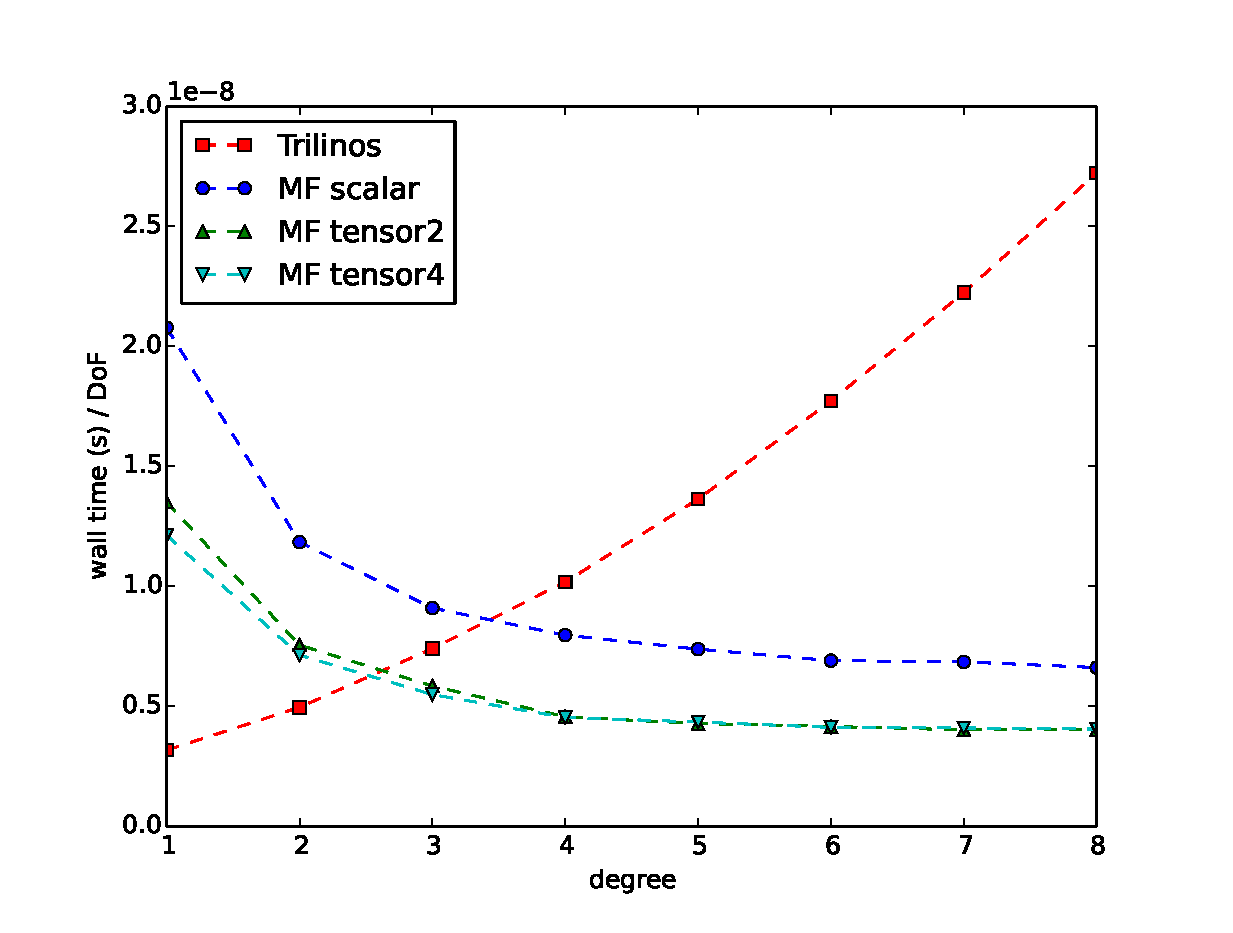
\includegraphics[width=\textwidth]{Emmy_RRZE_timing.eps}
      \caption{vmult}
  \end{subfigure}
  \begin{subfigure}[b]{0.49\textwidth}
      \centering
      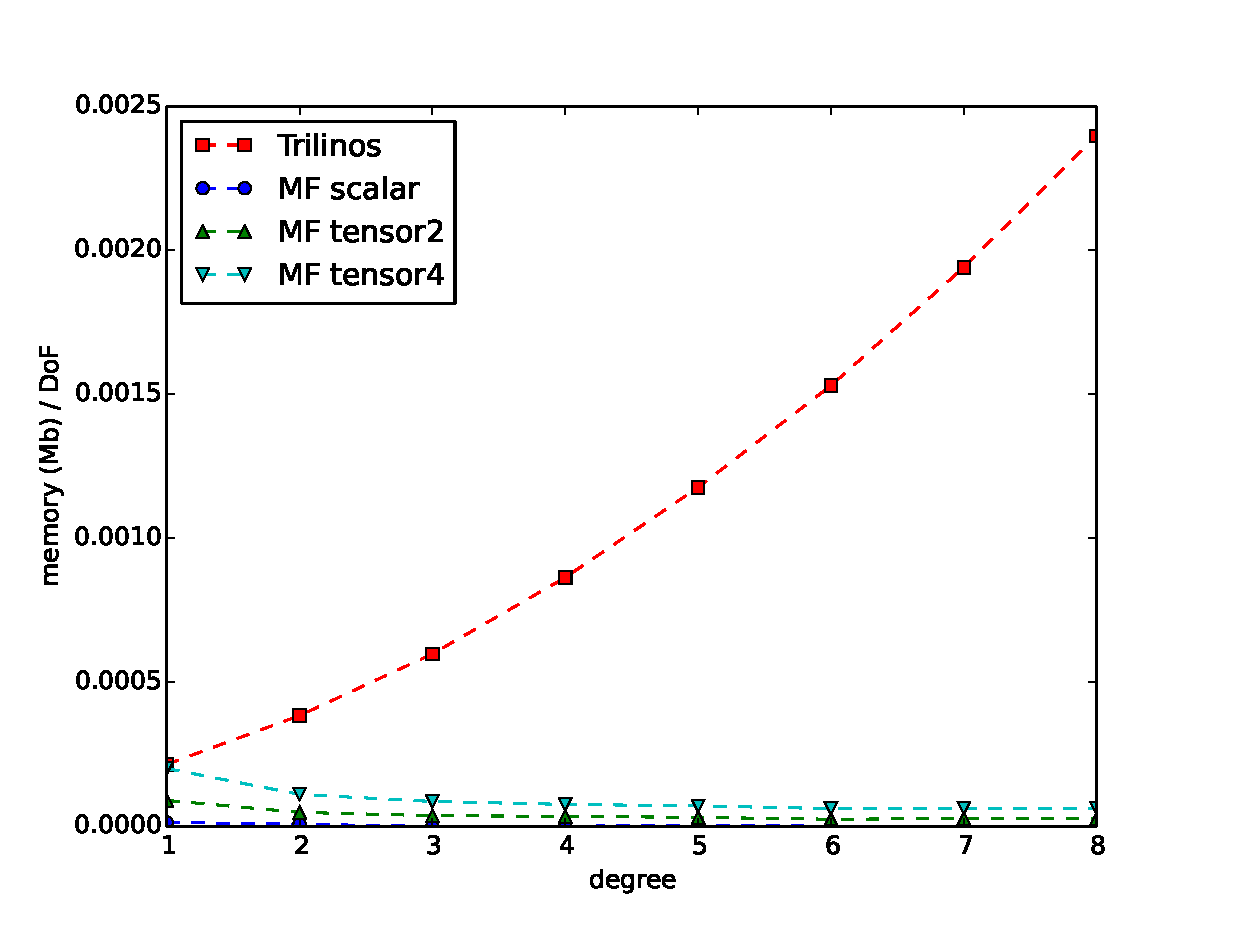
\includegraphics[width=\textwidth]{Emmy_RRZE_memory.eps}
      \caption{memory consumption}
  \end{subfigure}
  \caption{Heterogeneous 2D large-strain example (Emmy cluster, RRZE).}%
  \label{fig:benchmark_2d_miehe}
\end{figure}

\begin{figure}[!ht]
  \centering
  \begin{subfigure}[b]{0.49\textwidth}
      \centering
      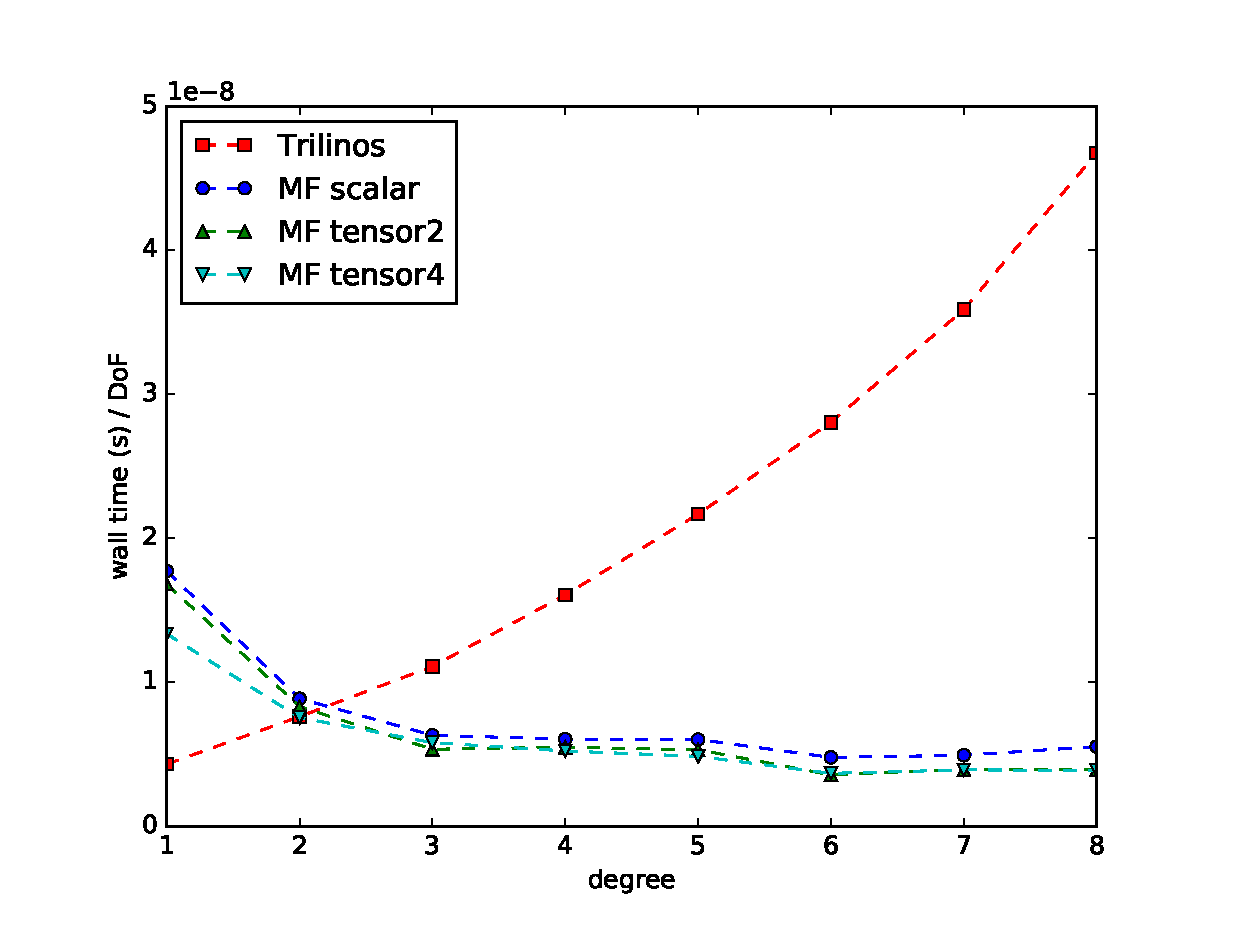
\includegraphics[width=\textwidth]{IWR_timing.eps}
      \caption{vmult}
  \end{subfigure}
  \begin{subfigure}[b]{0.49\textwidth}
      \centering
      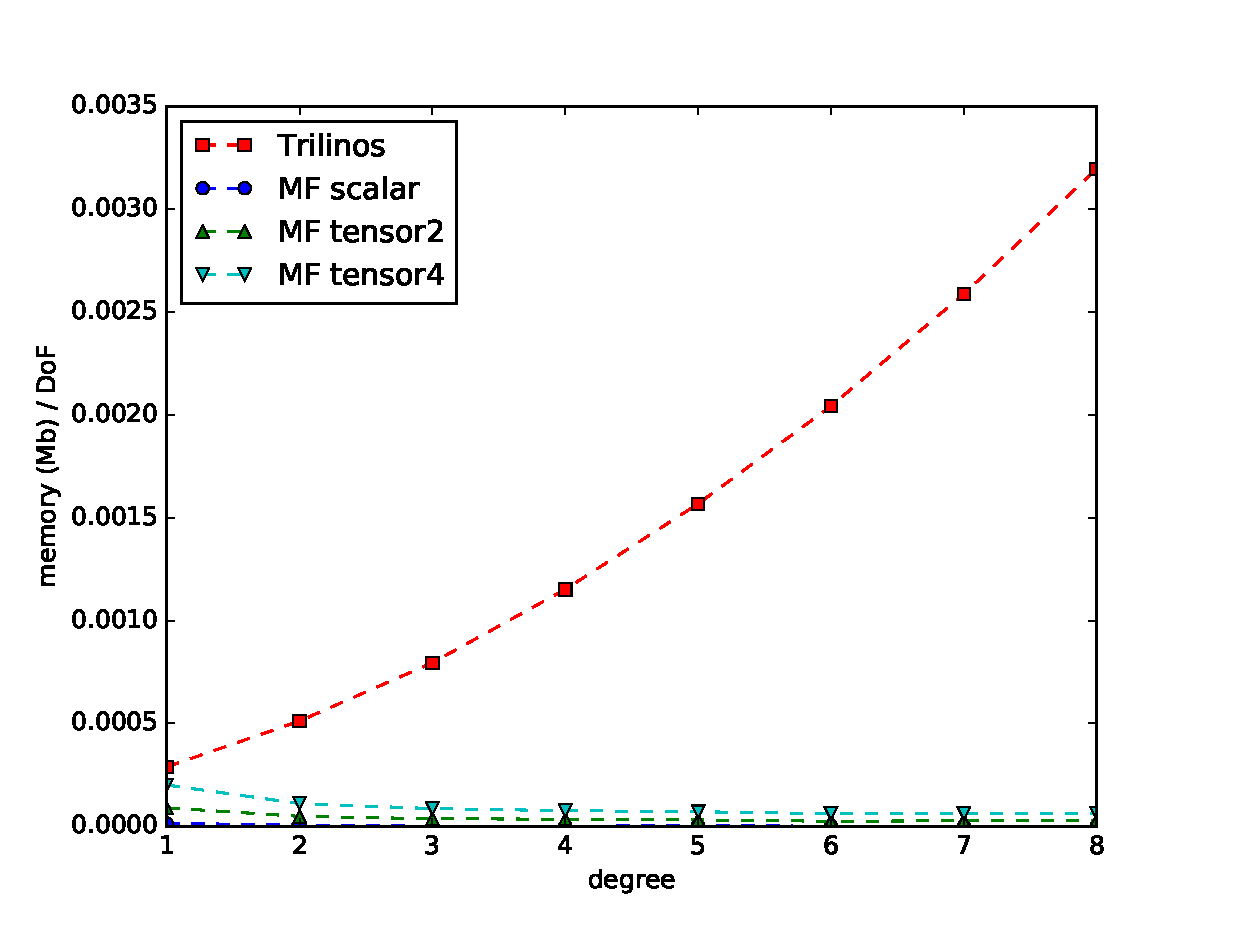
\includegraphics[width=\textwidth]{IWR_memory.eps}
      \caption{memory consumption}
  \end{subfigure}
  \caption{Heterogeneous 2D large-strain example (IWR cluster).}%
  \label{fig:benchmark_2d_miehe_IWR}
\end{figure}


TODO: add new results from Cook's and some matrix-inclusion (matrix-pore).
Elliptical holes are easier as we don't need heterogeneous operator.

\section{Summary and Conclusions}

TODO: summarize results, good/bad, where can be applied,...
Bio-med fluid-structure ?

\bibliographystyle{elsarticle-num}
\bibliography{bibliography}

\end{document}
